\begin{figure}[!ht]
	\setlength{\resLen}{1.6in}
	\addtolength{\tabcolsep}{-4pt}
	\footnotesize
	\begin{tabular}{c|c}
		Synthetic data & Real data\\
		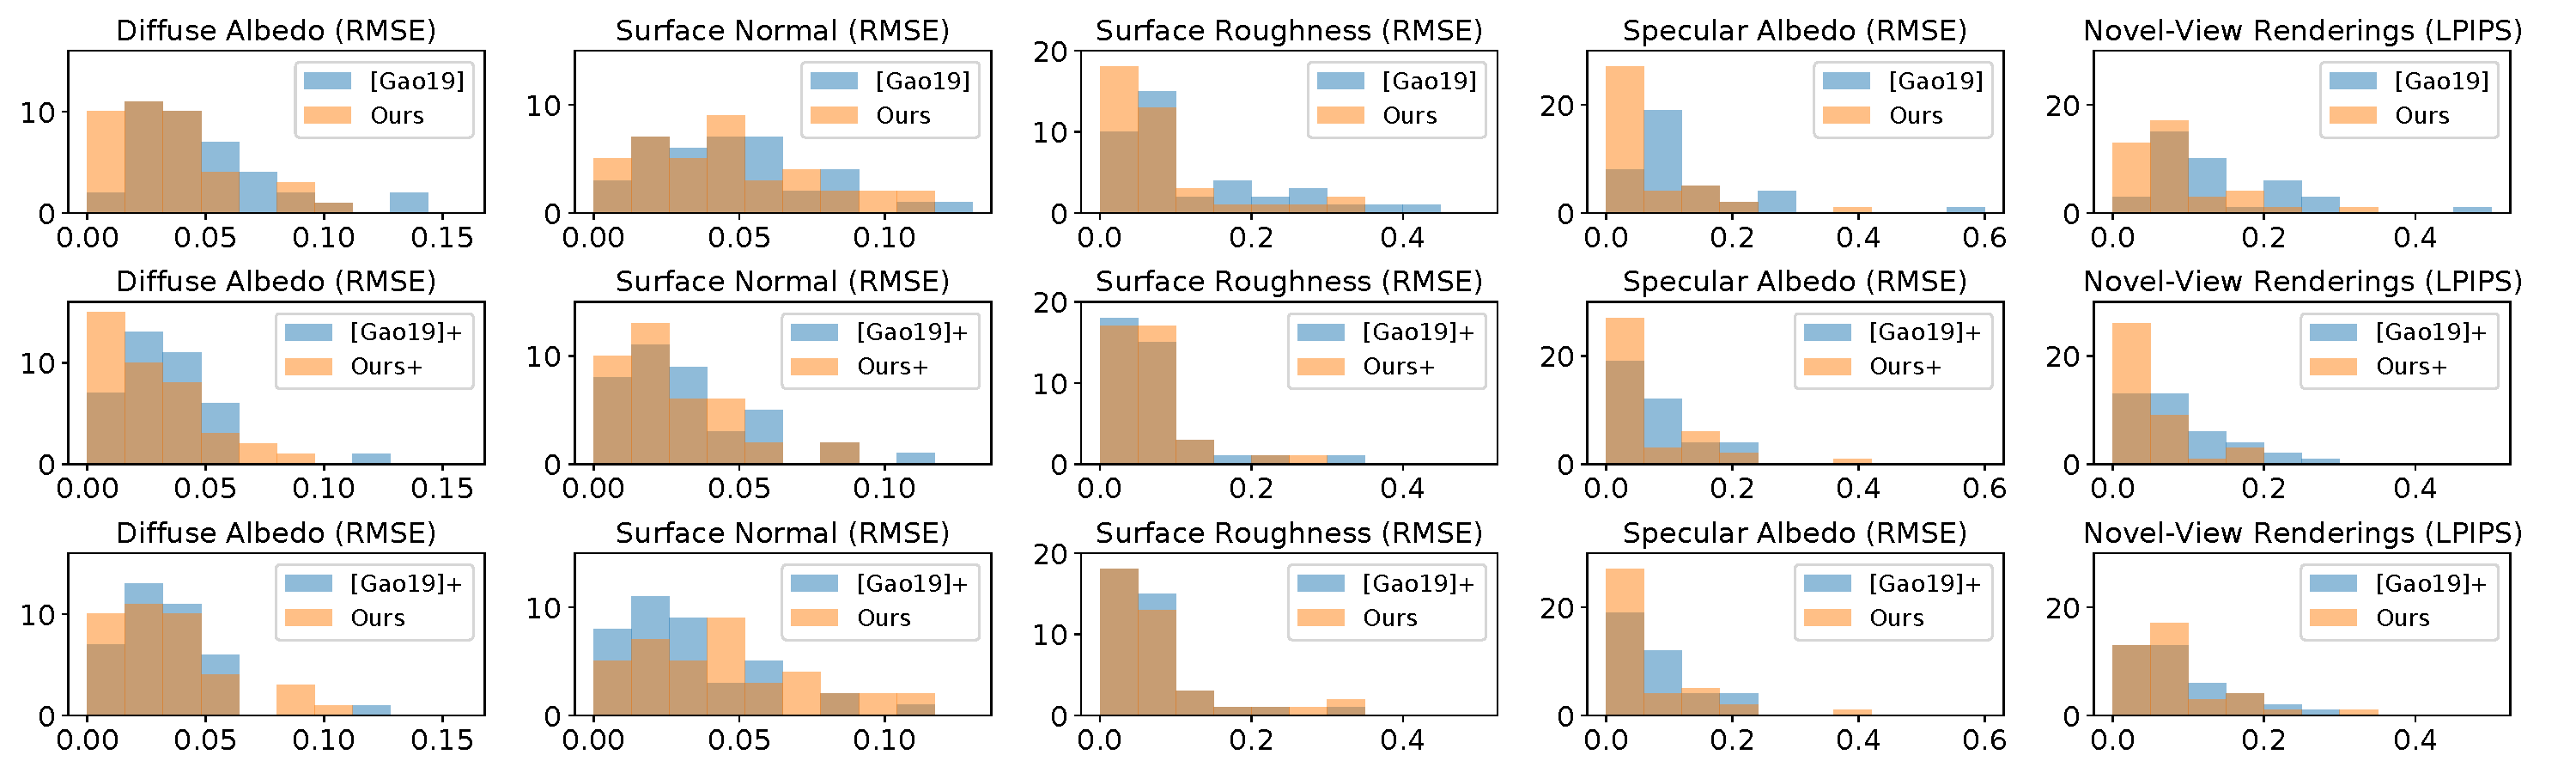
\includegraphics[height=\resLen]{svbrdf/results/rmse/hist_fake.pdf} &
		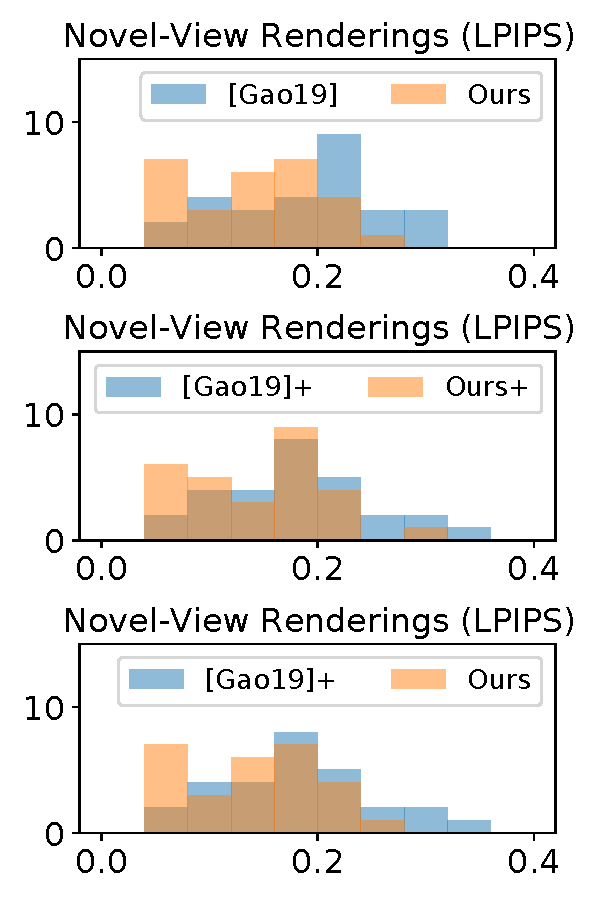
\includegraphics[height=\resLen]{svbrdf/results/rmse/hist_real.pdf}\\[-4pt]
	\end{tabular}
	\caption[Performance statistics]{\label{fig:svbrdf:rmse}
		\footnotesize \textbf{Performance statistics} of Gao \cite{gao2019deep} and our method.
		For each technique, we compute (i) the Learned Perceptual Image Patch Similarity (LPIPS) metric between renderings of the output SVBRDF maps and the reference images for 40 \emph{real} and 30 \emph{synthetic} examples; and (ii) the root-measure-square error (RMSE) of the inferred maps for the \emph{synthetic} examples.
		For both metrics, a lower score indicates a better accuracy.
		Using identical initializations, our technique (``Ours'' and ``Ours+'') outperforms Gao's (``[Gao19]'' and ``[Gao19]+'') consistently for both real and synthetic examples, as demonstrated in the top and the middle row.
		Furthermore, our technique with constant initializations (``Ours'') has a similar performance with Gao's method initialized using Deschaintre's \cite{deschaintre2019flexible} direct predictions (``[Gao19]+'') on the synthetic examples and outperforms the latter on the real examples, as shown on the bottom.
	}
\end{figure}
